\documentclass[12pt]{article}
\usepackage{fouriernc}
\usepackage{graphicx}
\usepackage{xcolor}
\usepackage[bookmarks=true,colorlinks=true,linkcolor=blue]{hyperref}

\begin{document}
\vspace{-1ex}
\noindent{}The Rockstar Halo Finder\\
\noindent{}Most code: Copyright \textcopyright{}2011-2016 Peter Behroozi\\
\noindent{}License: GNU GPLv3\\
\noindent{}Science/Documentation Paper: \url{http://arxiv.org/abs/1110.4372}\\

\tableofcontents
\newcommand{\ttt}[1]{\texttt{#1}}

\section{Compiling}
   If you use the GNU C compiler version 4.0 or above on a 64-bit machine,
   compiling should be as simple as typing ``\texttt{make}'' at the command prompt.
   If you need HDF5 support to read in snapshots, use ``\ttt{make with\_hdf5}''.

   Rockstar does not support compiling on 32-bit machines and has not been
   tested with other compilers.  Additionally, Rockstar does not support
   non-Unix environments.  (Mac OS X is fine; Windows is not).

\section{Running}
   \subsection{Quick start (single snapshot, single CPU)}
      Several example configuration files have been provided.  If you have a
      small simulation file and you'd like to run Rockstar on a single processor
      to test its output, edit the file ``\texttt{quickstart.cfg}'' and change the file
      format to one of \texttt{ASCII}, \texttt{GADGET}, \texttt{AREPO}, \texttt{ART}, 
      or \texttt{TIPSY} to match your simulation file.  If you use the \texttt{ART} option,
      only PMss files are currently supported.  (PMcrs files, which do not include particle IDs
      explicitly, are not supported).

      If you use \texttt{ASCII}, \ttt{ART}, or \ttt{TIPSY}, you will additionally have to set
      the particle mass; if you use \ttt{ASCII} or \ttt{TIPSY}, you will also have to
      set parameters for the cosmology and box size.

      If you use \texttt{GADGET}, you should check to make sure that the length
      and mass conversion multipliers are correct (\ttt{GADGET\_LENGTH\_CONVERSION} and
      \ttt{GADGET\_MASS\_CONVERSION}) to convert Gadget internal units to comoving Mpc/h
      and M$_\odot$/h.
      
      Note that \texttt{GADGET} only works with the binary GADGET formats.  For GADGET
      as well as AREPO HDF5 snapshots, use \texttt{AREPO} for the file format.  You will then have to
      set \ttt{AREPO\_LENGTH\_CONVERSION} and
      \ttt{AREPO\_MASS\_CONVERSION} to convert internal snapshot units to comoving Mpc/h
      and M$_\odot$/h, respectively.  Make sure to compile Rockstar with ``\ttt{make with\_hdf5}'';
      otherwise, the code will not accept these config options.

      If you use \ttt{TIPSY}, you should set the length and velocity
      conversion multipliers (\texttt{TIPSY\_LENGTH\_CONVERSION} and \texttt{TIPSY\_MASS\_CONVERSION})
      to convert Tipsy internal units to comoving Mpc/h and physical km/s.
      Note that Tipsy format is in a \textit{beta stage of support}---please contact
       me if you have issues!
       
       One final important variable to set is the force resolution of the simulation:
\begin{verbatim}
      FORCE_RES = <force res. of sim., in Mpc/h; default 0.003>
\end{verbatim}
	Halos whose centers are closer than \texttt{FORCE\_RES} are usually noise, and are subject to stricter removal tests than other halos.

      Then, you can run Rockstar:
      \begin{verbatim}
      ./rockstar -c quickstart.cfg <particle file>
\end{verbatim}      
      Note that periodic boundary conditions are \textbf{not} assumed for a single-cpu
      run.  (For that, see the next section, \S \ref{s:parallel_io}).

\begin{figure}
\vspace{-11ex}
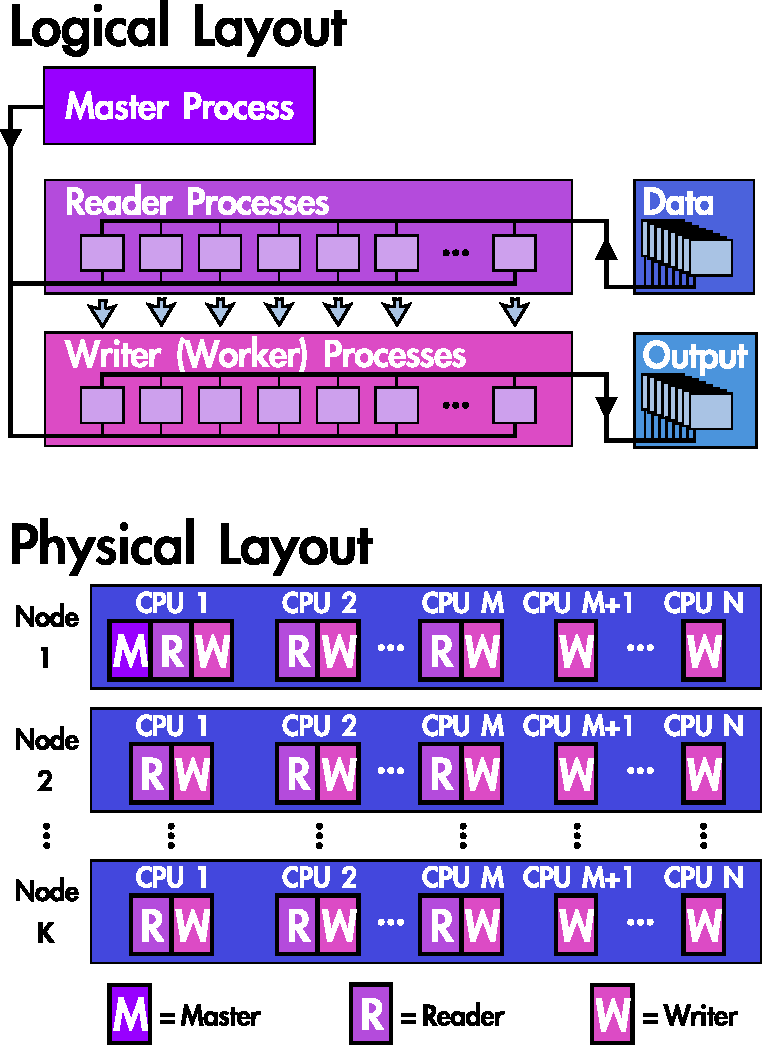
\includegraphics[width=0.8\columnwidth]{rockstar_layout.pdf}
\caption{\textbf{Logical Layout of Parallel Processing}: One master process controls multiple reader and writer (worker) processes.  The reader processes are responsible for loading data and rearranging it into rectangular volumes according to the number of writers.  The writer processes receive data from the readers, analyze it for halos, and write output catalogs to one or more files.  \textbf{Physical Layout}: Every CPU should contain one writer process, since this is where the bulk of the analysis time is spent.  The master process consumes very little CPU power, and so can easily be accommodated by the first CPU.  The reader processes also consume very little CPU power; however, they require enough memory to load in all the particle data.  For this reason, they should be distributed evenly across all the nodes.  Rockstar has several configuration parameters to help with launching the right number and the right type of tasks per node; see \S \ref{s:parallel_io}.}
\label{f:layout}
\end{figure}

\subsection{More Complete Setup (multiple snapshots/input files/CPUs)}
\label{s:parallel_io}
      Note: Rockstar does \textit{not} use MPI for its parallelization.  As such,
      there should be no headaches with finding a working MPI installation
      to use. :)

      For running on multiple snapshots or simulations with multiple input
      files per snapshot, Rockstar uses a master process to direct the
      order of processing steps and several client processes to do the
      actual work (see Fig.\ \ref{f:layout}).

      For historical reasons, enabling Rockstar to run on multiple input files,
      multiple snapshots, or multiple CPUs is controlled by setting the following ``Parallel
      IO'' option in the config file:
\begin{verbatim}
      	 PARALLEL_IO = 1
\end{verbatim}
      Besides setting the file type and conversion options in the previous section, 
      several more options are necessary in the configuration file to specify
      filenames, paths, and information about the number of processes you want
      to use.

      By default, the number of reading tasks is set to the number
      of files being read for each simulation snapshot:\footnote{If the number of blocks is more than the number of CPUs you wish to use, then you should also specify: \texttt{NUM\_READERS = $<$number of CPUs$>$}}
\begin{verbatim}
         NUM_BLOCKS = <number of files per snapshot>
\end{verbatim}
      You will also have to provide information on where the data files are
      located.  To do so, you will have to set:
\begin{verbatim}
      	 INBASE = "/directory/where/files/are/located"
        FILENAME = "my_sim.<snap>.<block>"
\end{verbatim}
      In this example, ``\texttt{my\_sim}'' should be the base of your simulation filename.
      For multiple snapshots, the text ``\texttt{$<$snap$>$}'' will be automatically replaced
      by the snapshot number, and the text ``\texttt{$<$block$>$}'' will be automatically
      replaced by the block number (0 to \texttt{NUM\_BLOCKS}-1).  To specify the range
      of snapshot numbers, you may set
\begin{verbatim}
         NUM_SNAPS = <total number of snapshots>
         STARTING_SNAP = <first snap> #defaults to 0
\end{verbatim}  
      If you have nonstandard names for your snapshots (e.g., ``001'' instead of
      ``1''),\footnote{Since GADGET always uses ``001'' instead of ``1'' for its snapshot numbers, Rockstar will automatically use the correct formatting without needing a snapshot filename list if the particle file type is \texttt{GADGET} or \ttt{AREPO}.} you may create a text file with one snapshot name per line and set:

\begin{verbatim}
         SNAPSHOT_NAMES = </path/to/snapshot names>
\end{verbatim}
      This will automatically override the number of snapshots \textit{and} the starting
      snapshot, if specified.  You may do the same thing for the block names,
      too:
\begin{verbatim}
         BLOCK_NAMES = </path/to/block names>
\end{verbatim}
      (Note that \texttt{NUM\_BLOCKS} should still be specified in this case, so that the
      server knows how many reader connections to accept).

      The number of writer (worker) tasks can be set to either 1 or a multiple of
      8. If set to 1, periodic boundary conditions are \textit{not} assumed; otherwise
      periodic boundary conditions \textit{are} assumed (see also the \texttt{PERIODIC} option
      in the full list of config options).  Usually, for best performance, you should set
      the number of writers to the total number of CPUs that you want to use for analysis:
\begin{verbatim}
      	  NUM_WRITERS = <number of CPUs>
\end{verbatim}
	You can also optionally specify an output directory where Rockstar will write all of its data products:
\begin{verbatim}
         OUTBASE = "/desired/output/path" # default is current directory
\end{verbatim}

      Starting Rockstar (under the default options) is then accomplished by
      first starting the server process:
      \begin{verbatim}
      	  /path/to/rockstar -c server.cfg
\end{verbatim}
      The server process will generate a file called ``\texttt{auto-rockstar.cfg}'' in the
      data output directory (\texttt{OUTBASE}) with contact information.

      You will then have to start \texttt{NUM\_READERS} (usually, \texttt{NUM\_BLOCKS})
      reader tasks and \texttt{NUM\_WRITERS} writer tasks (refer to Fig.\ \ref{f:layout} for task CPU assignment).  To simplify this process,
      there are two additional options you can set:
\begin{verbatim}
         FORK_READERS_FROM_WRITERS = 1
         FORK_PROCESSORS_PER_MACHINE = <number of processors per node>
\end{verbatim}
      The first option will automatically split off the reader tasks for you
      (which are idle most of the time) so that you only have to start the
      writer tasks.  The second option will automatically split each writer
      task you start into many copies (according to the number of processors
      you specify to use per node).  Thus, if these options are set properly, you would
      only have to start Rockstar running once on each compute node, instead of once
      per CPU.  The command to start the Rockstar reading/writing processes on each compute
      node would be:
\begin{verbatim}      
         /path/to/rockstar -c OUTBASE/auto-rockstar.cfg
\end{verbatim}
	As noted above, \texttt{OUTBASE} is the current working directory by default; however, if you change it in the config file, the \texttt{auto-rockstar.cfg} file will be written to that location as well.  Rockstar does not come with a command to start itself on many machines at the same time; however, the utilities which come with various MPI installations (e.g., \texttt{mpirun/mpiexec/ibrun}) are often suitable for doing so.  See \S \ref{s:full_example_scripts} for info about example startup scripts.

      In terms of memory usage, Rockstar will use about 60 bytes / particle
      \textit{maximum total} for a cosmological simulation.  Thus, if you have a
      $1024^3$ particle simulation and 2GB of memory available per processor, you should
      plan on using at least 32 CPUs in parallel.

      If Rockstar is terminated for any reason, it is easy to restart it where
      it left off.  Simply start the server process by running:
\begin{verbatim}
         /path/to/rockstar -c OUTBASE/restart.cfg
\end{verbatim}      
       Then, start client processes
      as you would normally.  Rockstar will resume analysis from the last incomplete
      snapshot.

\subsection{Inline Analysis for Simulations}
      For very large simulations, it is possible to have Rockstar run on particle snapshots as they become available.  If writing the snapshots to disk is not an option, Rockstar can also accept particle input from pipes (see \S \ref{s:input_formats}).  It is strongly recommended that you contact the authors for assistance before running an important simulation this way.

\subsection{Output}
\label{s:output}
Rockstar can output in many different formats (see \S \ref{s:output_formats} below).  If run in single-processor mode, halos are saved to a file called \texttt{halos\_0.0.ascii} with one line per halo.  If run in multi-processor mode, halos are saved to files called \texttt{out\_0.list}, \texttt{out\_1.list}, etc., with one file per particle snapshot.  Many halo properties are currently calculated by default:
\begin{itemize}
\item Halo masses at several radii: $M_\mathrm{vir}$, $M_{200b}$, $M_{200c}$, $M_{500c}$, $M_{2500c}$.  These masses always include any contributions from substructure.  Also, masses with higher density thresholds (e.g., 2500c) can sometimes be zero if the density of the halo never rises above the threshold.\footnote{Particles are assumed to have an effective radius of \texttt{FORCE\_RES} for the purposes of density calculations near the halo center.}  By default, only bound particles are included; see \S \ref{s:common_options} if this is not what you want.
\item Halo maximum circular velocity and velocity dispersion.
\item Halo radii: $R_\mathrm{vir}$ and the scale radius $r_s$, calculated both using profile fitting and using the Klypin $v_\mathrm{max}$ method.
\item Halo center positions and velocities.
\item Halo spin (both Bullock and Peebles) and angular momentum.
\item Halo shapes and principal axes, using the Allgood method (iterative, weighted by $1/r^2$), at both $R_\mathrm{vir}$ and $R_\mathrm{500c}$.  See \S \ref{s:common_options} for how to change the shape calculation method.
\item The ratio of halo kinetic to potential energy, and the center position and velocity offsets from the halo's bulk average position and velocity.
\end{itemize}

Information about each of the columns in both file types (including units) is available in the ASCII headers.  If you would like to calculate more halo properties, please see \S \ref{s:new_properties}.  



\subsection{Merger Trees}
	\label{s:merger_trees}
      By default, the output files for Rockstar include some basic descendant
      information for each halo.  However, it is strongly recommended that
      you use a more sophisticated package, such as Consistent Trees\\[1ex]
      \url{http://code.google.com/p/consistent-trees}\\[1ex] 
      to improve consistency
      between timesteps before using the descendant information for science
      purposes (e.g., calculating merger rates).  Rockstar includes a script
      to autogenerate configuration files for Consistent Trees (see the
      Consistent Trees README file for use).  It is \textit{very} important to use the
      same version of this script as the Rockstar version that you used for analysis.

\subsection{Host / Subhalo Relationships}
      By default, the output files for Rockstar do not include information
      about which halos are hosts (as opposed to subhalos).  This is because
      the consistent tree code (see \S \ref{s:merger_trees}, above) automatically
      calculates such relationships.  However, if you do not intend to use the
      merger tree code, then there is a utility included with Rockstar to
      postprocess the output halo catalogs (i.e., the \texttt{out\_*.list} files).  To
      compile, run ``\texttt{make parents}'' from the Rockstar source directory.  Then,
      run the following command
\begin{verbatim}
      	  /path/to/rockstar/util/find_parents out_XYZ.list <box_size>
\end{verbatim}
      on each halo catalog for which you want to find host halos.  Information
      about which halos are hosts and which are subs will be output as an
      extra column, the parent ID.  Host halos will have a parent ID of -1;
      subhalos will have a parent ID which corresponds to their host halo ID.
      Note that the files produced will \textit{not} be suitable for input into the
      merger tree code above.

\subsection{Lightcones}
      Lightcones are currently only supported with parallel IO (see options
      above).  To turn on lightcone support, set
\begin{verbatim}
         LIGHTCONE = 1
\end{verbatim}
      The scale factor will be automatically computed
      from the distance to the origin, which is set by
\begin{verbatim}
         LIGHTCONE_ORIGIN = (x,y,z) #default: (0,0,0)
\end{verbatim}
      If you want a lightcone created by joining two different fields of view
      from the same box, you will have to set the following options:
\begin{verbatim}
         LIGHTCONE_ALT_SNAPS = /path/to/second_lightcone_snapnames
         LIGHTCONE_ALT_ORIGIN = (x,y,z) #default: (0,0,0)
\end{verbatim}
      (The \texttt{LIGHTCONE\_ALT\_ORIGIN} option translates all particles in the second
      field of view from (x,y,z) to the first \texttt{LIGHTCONE\_ORIGIN}.)  If using two
      fields of view, it is assumed that they have equal numbers of input files;
      \texttt{NUM\_BLOCKS} should be set to the combined total number of input files.

      If you have more than two fields of view from the same box, you will
      have to make sure that their positions are already translated
      appropriately so that they can be joined/unioned together without any
      overlap issues.  In this case, you should not set any of the ALT lightcone
      options.  Additionally, you should set ``\texttt{IGNORE\_PARTICLE\_IDS = 1}'' so as
      to prevent confusion with the same particle ID appearing multiple times.

\subsection{Controlling Output Formats}
\label{s:output_formats}
      Rockstar can currently output in either ASCII or binary formats.
      You can control the output directory for halo catalogs by setting:
\begin{verbatim}
         OUTBASE = "/desired/output/path" # default is current directory
\end{verbatim}
      By default, both binary and ASCII catalogs are printed.  This is set by
\begin{verbatim}
         OUTPUT_FORMAT = BOTH # or "ASCII" or "BINARY"
\end{verbatim}
      However, as the binary outputs are required for generating merger trees,
      merger trees will \textit{not} be generated if you select the \texttt{ASCII} option.
      If you want merger trees but not the binary outputs (which take up
      lots of space), you can set the following option:
\begin{verbatim}
         DELETE_BINARY_OUTPUT_AFTER_FINISHED = 1
\end{verbatim}
      For the binary outputs, there is a 256-byte header (detailed in
      \texttt{io/io\_internal.h}) followed by a binary dump of the halo structures
      (see \texttt{halo.h}), followed by a binary dump of the particle ids in
      each halo (type \texttt{int64\_t}).  See the \texttt{load\_binary\_halos()} routine in
      \texttt{io/io\_internal.c} for an example of how to read in the binary files.

      To change the minimum particle size of output halos, set
\begin{verbatim}
          MIN_HALO_OUTPUT_SIZE = <minimum number of particles> #default: 20
\end{verbatim}
      Note that this option does \textit{not} specify the minimum number of particles
      bound within the virial or other halo radius.  Instead, it specifies the
      minimum number of particles which Rockstar identifies as uniquely assigned
      to that halo.  The virial mass can (and usually will) be much less.

      To avoid printing spurious halos, Rockstar excludes significantly 
      unbound objects by default.  To change the threshold of what is considered
      ``significantly unbound''---e.g., for studying tidal remnants, you may
      consider lowering the value of the following parameter:      
\begin{verbatim}
      	 UNBOUND_THRESHOLD = <minimum fraction of bound mass> #default: 0.5
\end{verbatim}
      Generally, this affects the halo mass function at the few percent level
      for halos of 100 bound particles or less (see the Rockstar science paper for details).

      Rockstar does not by default output full particle information to
      save space.  In order to turn on this capability, set
\begin{verbatim}
         FULL_PARTICLE_CHUNKS = <number of writers which will output particles>
\end{verbatim}
      to the desired number of writer processes which you want to output
      particles (i.e., something between 1 and \texttt{NUM\_WRITERS}) at every timestep.

      Alternately, you can choose to use the BGC2 binary output format, which
      records full particle information as well as some halo information for
      an entire snapshot.  In order to turn on this capability, set
\begin{verbatim}
         BGC2_SNAPNAMES = </path/to/snapshot_names>
\end{verbatim}
      Where the file contains a list of snapshots (formatted the same way as
      in \texttt{SNAPSHOT\_NAMES}, if you used that option) for which you want BGC2
      output.  Note that the BGC2 format is currently incompatible with processing
      lightcones.

      Once the BGC2 files have been generated, a short postprocessing step
      is necessary to bring them into full compliance with the BGC2 format specification (calculating
      subs/centrals, etc.).  You will need to compile the postprocessing
      code with
\begin{verbatim}
         make bgc2
\end{verbatim}
      Then, for every BGC2 snapshot you have generated, you will need to run
\begin{verbatim}
         /path/to/rockstar/util/finish_bgc2 -c rockstar.cfg -s <snap>
\end{verbatim}
      Note that particle coordinates in BGC2 files are automatically wrapped around
      box edges if periodic boundary conditions are enabled; this way, they
      always form contiguous regions.

      For additional useful source code to load in both the BGC2 and
      full-particle halo/particle formats, check the \texttt{examples/} subdirectory.

\subsection{Comparing to Published Mass Functions}

      By default Rockstar calculates halo and subhalo masses using particles from the surrounding friends-of-friends group with unbound particles removed.  This leads to halo masses which are very consistent for merger trees, but which are a few percent below published spherical overdensity (SO) calibrations.  For comparing to calibrated mass functions, the simplest approach is to generate BGC2 files (see \S \ref{s:output_formats}, above).  If you don't have software to read BGC2 files, you can use the BGC2 to ASCII converter supplied with Rockstar:
\begin{verbatim}
         /path/to/rockstar/util/bgc2_to_ascii -c rockstar.cfg -s <snap>
\end{verbatim}
You should then calculate mass functions from the resulting output; subhalos can be excluded by skipping halos which do not have \texttt{PID=-1}.


\subsection{Infiniband / Network Connectivity Notes}
      As particle transfer is usually a small fraction of the total analysis
      time, Rockstar performs well on pretty much any gigabit or faster network.

      If you have IP over Infiniband, Rockstar can use this natively.  If the primary
      server IP address is not for an Infiniband network, you may force Rockstar to use the
      Infiniband interface (e.g., ``\texttt{ib0}'') with the following config option:
\begin{verbatim}
         PARALLEL_IO_SERVER_INTERFACE = "ib0"
\end{verbatim}
      Rockstar supports IPv4 and IPv6 natively; addresses may be specified
      in either format.



\subsection{Full Configuration Options}
\label{s:full_options}

\subsubsection{Commonly-Used Options}
\label{s:common_options}
      For those options not mentioned directly above:
\begin{verbatim}
      	  MASS_DEFINITION = <"vir" or "XXXc" or "XXXb" etc.> #default: vir
\end{verbatim}
      This lets you specify how you want masses calculated.  ``\texttt{vir}'' uses the
      formula from Bryan \& Norman (1998); a number plus "c" or "b" calculates
      masses relative to the critical or background density, respectively.
      (E.g. ``\texttt{200b}'' or ``\ttt{200c}'', or even fractional values like ``\texttt{100.5c}'').
      Changing the main mass definition will also change the halo radius at which most other
      properties are calculated (e.g., $v_\mathrm{max}$, spin, shape, etc.).
      
      Besides the main mass definition, you can specify four other halo mass definitions to calculate,
      in \texttt{MASS\_DEFINITION2} through \texttt{MASS\_DEFINITION5}.  The syntax for these is
      identical to that for \texttt{MASS\_DEFINITION}; the defaults are listed in \S \ref{s:output}.  Note that
      for very low density thresholds (e.g., $<150$b), you may have to increase the value of \texttt{FOF\_LINKING\_LENGTH} below to obtain accurate masses.

      By default, all masses are calculated from FOF groups after
      unbound particles are removed.  This is appropriate for merger trees,
      where halos/subhalos need to be treated identically for consistency
      across timesteps.  However, if you are calculating \textit{mass functions},
      you will want to use spherical overdensities including unbound particles
      and particles which may exist outside of the FOF group for the halo.
      To enable these strict SO masses, use
\begin{verbatim}
          STRICT_SO_MASSES = 1 #default: 0
\end{verbatim}
      The resulting masses will be present in the auxilliary mass columns
      (columns 20-24) of the \texttt{out\_*.list} files.  This option is only available in parallel processing mode (\S \ref{s:parallel_io}).  If computing mass functions for snapshots widely separated in redshift, you may also wish to disable temporal halo finding (i.e., using information from previous snapshots to determine host/sub relationships):
\begin{verbatim}
          TEMPORAL_HALO_FINDING = 0 #default: 1
\end{verbatim}

	Shape calculations are by default performed with the Allgood method.  If you wish to change this, you can specify
\begin{verbatim}
          WEIGHTED_SHAPES = 0 #default: 1
\end{verbatim}
	which will calculate the mass tensor without weighting by $1/r^2$.  In addition, if you do not want the shapes to be calculated iteratively, specify
\begin{verbatim}
          SHAPE_ITERATIONS = 1 #default: 10
\end{verbatim}
	This setting specifies the maximum number of shape calculation iterations to perform.

      Options to set the base cosmology are available:
\begin{verbatim}
          SCALE_NOW = <current cosmological scale factor>
          h0 = <hubble constant today> # in units of 100 km/s/Mpc
          Ol = <Omega_Lambda> # in units of the critical density
          Om = <Omega_Matter> # in units of the critical density
\end{verbatim}
      These cosmology options are only relevant if one is reading from an ASCII
      or TIPSY particle file.  (For TIPSY, the \texttt{SCALE\_NOW} parameter may be
      omitted).  For other data formats, these values are \texttt{automatically
      overwritten} with values in the particle data files.

       Non-LCDM equations of state are also available.  Since none of the particle input formats include a standard way of specifying these, the equation of state must be specified in the config file:
\begin{verbatim}      
          W0 = <W_0> # dark energy equation of state at z=0
          WA = <W_A> # scaling of DE equation of state with scale factor.
\end{verbatim}
	By default, these are set to \texttt{W0=-1} and \texttt{WA=0}.

      It is not necessary to specify the particle mass for GADGET2 files, but it is necessary for all other file types:
\begin{verbatim}
          PARTICLE_MASS = <mass of each particle> #in Msun/h
\end{verbatim}

      However, for GADGET2 files, you will need to specify the conversion to
      Rockstar's internal length (comoving Mpc/h) and mass (M$_\odot$/h) units:
\begin{verbatim}
          GADGET_MASS_CONVERSION = <conversion from GADGET units to Msun/h>
          GADGET_LENGTH_CONVERSION = <conversion from GADGET units to Mpc/h>
\end{verbatim}
      Usually, these will be \texttt{1e10} (mass conversion) and either \texttt{1} or
      \texttt{1e-3} (length conversion for Mpc/h and kpc/h, respectively).

      Similarly, for TIPSY files, you will need to convert lengths and
      velocities to comoving Mpc/h and physical km/s:
\begin{verbatim}
          TIPSY_LENGTH_CONVERSION = <conversion from TIPSY units to Mpc/h>
          TIPSY_VELOCITY_CONVERSION = <conversion from TIPSY units to km/s>
\end{verbatim}
      To disable periodic boundary conditions (only applicable for \texttt{PARALLEL\_IO}),
      you can set:
\begin{verbatim}      
          PERIODIC = 0
\end{verbatim}
      Note that setting this to 1 does \textit{not} enable periodic boundary conditions
      for single-processor halo finding.

      For ASCII particle data, it is necessary to specify the box size:
\begin{verbatim}
      	  BOX_SIZE = <side length of cosmological box in comoving Mpc/h>
\end{verbatim}

      To run postprocessing scripts after each snapshot finishes, you can use
      the \texttt{RUN\_ON\_SUCCESS} config option:
\begin{verbatim}
      	  RUN_ON_SUCCESS = "/path/to/myscript"
\end{verbatim}
      The script will be executed with two arguments: the snapshot number
      followed by the snapshot name (only different if specified via the
      \texttt{SNAPSHOT\_NAMES} file).  If parallel processing is enabled, it
      will run in the background on the first compute node only.
      
      To run postprocessing scripts in parallel (i.e., one per writer task), you can use 
\begin{verbatim}
      	  RUN_PARALLEL_ON_SUCCESS = "/path/to/myscript"
\end{verbatim}
	The script will be executed by each writer task, and further analysis will pause
	until all the scripts finish.  The script will be given five arguments, which are the current snapshot
	number, the total number of snapshots, the writer task number (0 to \texttt{NUM\_WRITERS}-1),
	the total number of writers, and the path to the Rockstar configuration file.  Spaces in the pathname must be escaped, because the script is run via the shell instead of executed directly.

	To restart Rockstar from a specific snapshot, use
\begin{verbatim}
      	  RESTART_SNAP = <snapshot number> #default: 0
\end{verbatim}
	This will resume analysis with the assumption that all snapshots previous to \texttt{RESTART\_SNAPSHOT} have been analyzed.

\subsubsection{Rarely-used Options}
\begin{verbatim}
      	  GADGET_SKIP_NON_HALO_PARTICLES = <0 or 1> #default = 1
\end{verbatim}
      By default, Rockstar only considers dark matter particles; the preceding
      option can be set to 0 to force consideration of other particles as well
      in GADGET2 files.  The default halo particle type in GADGET is 1; however,
      if you need to change this, you can use the following option:
\begin{verbatim}
          GADGET_HALO_PARTICLE_TYPE = <0 to 5> #default = 1
\end{verbatim}
      Note that Rockstar has no current support for multiple particle masses.  A beta version of Rockstar with support for multi-mass particles is available on request from the authors.
\begin{verbatim}
      	  RESCALE_PARTICLE_MASSES = <0 or 1> #default 1
\end{verbatim}
      If only dark matter particles are used from GADGET2 files in a simulation
      which also includes gas particles, it is necessary to rescale the particle
      masses so as to preserve the correct matter density; setting this option
      tells Rockstar to do so.

      If for some reason your simulation data has inconsistent or duplicate
      particle IDs, you can set the following option to prevent problems with
      halo finding:
\begin{verbatim}
          IGNORE_PARTICLE_IDS = 1
\end{verbatim}
      Note that in this case, merger trees are disabled.

      As mentioned above, Rockstar requires one master server accessible by
      all reader and writer tasks.  The server does not require access to any
      data files, but it must be of the same architecture as the reader/writer tasks.  In order to contact the master server, the reader/writer tasks need to know its address, specified by the following two
      options in the config file:
\begin{verbatim}
      	 PARALLEL_IO_SERVER_ADDRESS = <server address> #default: auto
      	 PARALLEL_IO_SERVER_PORT = <server port> #default: auto
\end{verbatim}
      The server port should be in the range 1025-65000, and it should be
      unblocked by the server firewall.  Alternately, you may specify
      ``\texttt{auto}'' for both the server address and the server port.  In this case,
      once you launch the server process, it will write to a file called
      ``\texttt{auto-rockstar.cfg}'' in the launch directory (or the directory that
      \texttt{OUTBASE} is set to).  This file will contain updated settings with
      the machine name and port for the server, which you can then use
      to launch the reader/writer tasks.  To force Rockstar to use a
      specified interface (useful for machines on multiple networks),
      you can use:
\begin{verbatim}
      	 PARALLEL_IO_SERVER_INTERFACE = <interface name> #ib0, for example
\end{verbatim}
      Since analysis tasks have to acquire particle data from reading tasks,
      the analysis tasks need to be contactable by the reading tasks.  You
      should choose a port number for the analysis tasks which is distinct
      from the server port above:
\begin{verbatim}
          PARALLEL_IO_WRITER_PORT = <port from 1025-65000>
\end{verbatim}
      If you have a firewall, you will have to open this port for access
      \textit{as well as} the $N$ ports above this port, where $N$ is the number of
      writer tasks you are running per compute node.

      The following options determine details of the halo finding.  To tell
      Rockstar to calculate halo radii as well as Vmax, Rvmax, and other
      halo properties from the *unbound* particles, set the following option
      to 0:
\begin{verbatim}
          BOUND_PROPS = <0 or 1> #default 1
\end{verbatim}
	This is likely not what you want if you are calculating mass functions; you should use \texttt{STRICT\_SO\_MASSES} instead (\S \ref{s:common_options}).

      To change the default FOF refinement fraction (see the Rockstar paper),
      change:
\begin{verbatim}
          FOF_FRACTION = <FOF refinement fraction> #default 0.7
\end{verbatim}
      To change the default 3D FOF linking length, set:
\begin{verbatim}
          FOF_LINKING_LENGTH = <FOF linking length> #default 0.28
\end{verbatim}
	This is generally only necessary to increase if trying to find halos with very low spherical overdensity thresholds.

      To change the minimum (internal) number of particles considered to be
      a halo seed, change:
\begin{verbatim}
          MIN_HALO_PARTICLES = <minimum number of halo particles> #default: 10
\end{verbatim}

      See also \texttt{MIN\_HALO\_OUTPUT\_SIZE} in \S \ref{s:output_formats}.


      To specify your own load-balancing distribution, you can use the
      \texttt{LOAD\_BALANCE\_SCRIPT} option.  There is an example of such a script in
      the scripts directory; to use, set the \texttt{LOAD\_BALANCE\_SCRIPT} option to
      \begin{verbatim}
      "perl /path/to/rockstar/scripts/sample_loadbalance.pl"
      \end{verbatim}
      The data given to the load-balancing script are the number of writer tasks,
      the recommended dimensional divisions,
      the box size, the scale factor, as well as the IP addresses and ports
      of all the writer tasks.  The script is expected to reoutput the
      information for each writer task along with an additional set of six
      numbers specifying the boundary region (min\_x, min\_y, min\_z) to
      (max\_x, max\_y, max\_z).  The boundary region \texttt{must} be contained within
      the box size in each dimension; the boundary regions are also assumed not to
      be overlapping (it is up to your script to check this).

\subsection{Full Example Scripts}
\label{s:full_example_scripts}
      For full example configuration files, used for running on the Bolshoi
      and Consuelo simulations, see \texttt{scripts/pleiades.cfg} or \texttt{scripts/ranger.cfg}.

      For the example PBS submission script used to run the halo finding on
      Pleiades, see \texttt{scripts/pleiades.pbs}; for Ranger, see \texttt{scripts/ranger.pbs}.

\section{Extending Rockstar}

	Rockstar is written in C, and requires no external libraries by default.  Please see the \texttt{SOURCE\_LAYOUT} file for a brief description of all source code files.

\subsection{Adding More Configuration Parameters}
      Config parameters are defined in \texttt{config.template.h}.  The syntax is
\begin{verbatim}
          <type>(VARIABLE_NAME, DEFAULT_VALUE)
\end{verbatim}      
      where \texttt{$<$type$>$} is one of
      ``\texttt{string}'' (\texttt{char *}), ``\texttt{integer}'' (64-bit signed integer, i.e., \texttt{int64\_t}),
      ``\texttt{real}'' (\texttt{double}), or ``\texttt{real3}'' (\texttt{double[3]}).

      Config parameters added here will be globally visible in the code
      and automatically interpreted from the config file.  The default
      value will be assigned if the config file does not include the
      variable.
      
\subsection{Adding More Input Formats}
\label{s:input_formats}
	If you run Rockstar through YT (\url{http://yt-project.org/}), you may find that your desired input format is already supported.  Alternatively, if you have existing code to read in particles and output in binary GADGET or ART format (not including HDF5), you can use named pipes to directly communicate the data to Rockstar.  This technique is also useful for analyzing simulation data as the simulation is running.  You can use the script in \texttt{scripts/mkpipes.pl} to make named pipes; you should ask it to make as many named pipes as you have files per snapshot.  Then, you would set \texttt{FILENAME = /path/to/pipe.$<$block$>$}.  To get data into the pipes, you would simply open and print to them like normal files (or use output redirection from \texttt{stdout}).  For example, you could have one script per pipe, which would be responsible for writing one block of particles to the pipe from each snapshot.  Since write operations to named pipes will pause execution of the writing program if the pipe has reached its buffer capacity (typically 4KB), the scripts will automatically pause until Rockstar has finished processing an entire snapshot and is ready to read in new data.
	
For highest efficiency, it is appropriate to copy one of the existing \texttt{io/io\_*.c} routines and modify it to accept your input format directly.  You will have to define a routine that looks like:
\begin{verbatim}
    void load_particles_mytype(char *filename, struct particle **p, 
	       				  int64_t *num_p)
\end{verbatim}					  
This routine should add the number of particles in the file to \texttt{num\_p} and grow the particle structure appropriately, e.g.,
\begin{verbatim}
     check_realloc_s(p[0], sizeof(struct particle), num_p[0] + num_new_p);
\end{verbatim}
Note that \texttt{check\_realloc\_s()} is defined in \texttt{check\_syscalls.h}.  It is generally a good idea to use the IO routines defined in that header, as they will automatically halt the program if they encounter any errors reading, writing, or opening files, making debugging much easier.  Routines helpful for reading Fortran-unformatted files and files encoded in a different endianness are available from \texttt{io/io\_util.h}.

The particle structure is very simple; it is described in \texttt{particle.h}.  Your routine should convert everything to Rockstar's internal units: i.e., comoving Mpc/h for positions and non-comoving km/s for peculiar velocities.  Your routine should also set as many config variables as possible (e.g., \texttt{BOX\_SIZE}, \texttt{PARTICLE\_MASS}, cosmology, current scale factor, etc.) from the data header, as that will reduce the chance for errors in the analysis from incorrectly-supplied config variables.

Once you have created a new \texttt{io/io\_mytype.c} file, you should create a corresponding header file and include it in \texttt{io/meta\_io.c}.  You can then add a new condition in the \texttt{read\_particles()} routine in \texttt{io/meta\_io.c} to call your code when the \texttt{FILE\_FORMAT} variable matches your filetype.  Finally, you should add the new \texttt{io/io\_mytype.c} file to the \texttt{Makefile} so that it gets compiled along with the other Rockstar source code.

If you think your code may be useful for others, please consider submitting it as a patch to the authors.  Others will no doubt appreciate it!

\subsection{Adding More Output Formats}

Halos are output in the \texttt{output\_halos()} routine in \texttt{io/meta\_io.c}.  Halos are stored in the \texttt{halos} array, for which the structure is defined in \texttt{halo.h}.  Particles are stored in the \texttt{p} array, for which the structure is defined in \texttt{particle.h}.  It is best to use the \texttt{output\_binary()} routine from \texttt{io/io\_internal.c} as a starting template for outputting halo and particle data.

\subsection{Adding More Halo Properties}
\label{s:new_properties}
All halo properties are calculated in \texttt{properties.c}, in the routine\\ \texttt{\_calc\_additional\_halo\_props()}.  All particles associated with the current halo being analyzed are in the \texttt{po} array, which is of type \texttt{struct potential} (defined in \texttt{potential.h}); particles in the array are sorted by distance from the halo center.  You may either add calculations directly in the main particle loop in \texttt{\_calc\_additional\_halo\_props()}, or you may decide to create your own particle loop as a separate routine.  If the latter case, don't forget to honor the option to skip over unbound particles unless your calculation always needs to include them; otherwise, you may get strange results for subhalos.

You may store your calculated values by extending the halo structure, defined in \texttt{halo.h}.  To print out the new properties, you should modify \texttt{gen\_merger\_catalog()} in \texttt{io/meta\_io.c}.  As with new input formats, if you think your code may be useful for others, please consider submitting it as a patch to the authors.
\end{document}
